\documentclass[12pt]{article}

%% - - - page formatting
% \renewcommand{\baselinestretch}{2.0}
\usepackage[doublespacing]{setspace}
\usepackage[margin=1in, left=1in, top = 1in, includefoot]{geometry} 
\usepackage[document]{ragged2e}
\setlength{\RaggedRightParindent}{2em}
\RaggedRight
\usepackage{indentfirst}
\setlength\footnotemargin{0em}
\usepackage{appendix}
\usepackage{endnotes}
\renewcommand{\theendnote}{\Roman{endnote}} 
\usepackage{enumerate}
\usepackage{enumitem}
\usepackage{float}

%% - - - Citations & References
\usepackage[style=apa]{biblatex}
% \addbibresource{./references.bib}
\bibliography{./references.bib}

\usepackage{hyperref}
\hypersetup{
    colorlinks = true,
    urlcolor = blue,
    citecolor = [rgb]{0, .121, .388},
    linkcolor = black,
    linkcolor = [rgb]{.349, 0, 0},
}

% personal preference :)
\let\oldcite=\cite
\let\oldtextcite=\textcite
\renewcommand{\cite}[1]{\textcolor[rgb]{0, .121, .388}{\oldcite{#1}}}
\renewcommand{\textcite}[1]{\textcolor[rgb]{0, .121, .388}{\oldtextcite{#1}}}

%% - - -  Math
\usepackage{mathtools}
\usepackage{algorithm}
\usepackage{algorithmic}

%% - - - Media
\usepackage{graphicx}
\usepackage[rightcaption]{sidecap}

\pagenumbering{roman}

%________________________________________________________________________________
\title{Shared Explanatory Frameworks for Function Learning and Category Learning in Humans}
\author{Matt Wetzel}
%________________________________________________________________________________


\begin{document}

% % % % % % % % % %
%
%   TITLE
%
% % % % % % % % % %
\maketitle
\pagebreak

\tableofcontents
\pagebreak

% - - - - - - - - - - - - - - - - - - - - - 
% - - - - - - - - - - - - - - - - - - - - - 



% % % % % % % % % %
%
%   CONTENT
%
% % % % % % % % % %

\section{Introduction}
\pagenumbering{arabic}

Our ability to successfully navigate through and understand our environment necessitates a sensitivity to the interrelationships between percepts, concepts, and events (both internal and external). For example, cooking a meal requires sensitivity to the functional relationships between temperature, quantity, and time, as well as the categorical relationships between ingredients and tastes. Much of the category learning (CL) literature has investigated the question of how categorical knowledge is acquired and generalized from and across percepts / concepts (\cite{kurtz2015human,ashby2005human}). Similarly, the function learning (FL) literature has focused on the question of how humans learn and extrapolate functional relationships between multiple continuously valued percepts / concepts (\cite{kalish2004population,busemeyer1997learning}). Despite being seemingly disparate literatures, both involve mapping relationships between variables, and many of the leading theoretical explanations of FL and CL leverage the same computational frameworks (\cite{busemeyer1997learning,lucas2015rational}). As such, the goals of the following paper are to (a) highlight the disparities and similarities between CL and FL, and (b) explore theoretical frameworks that provide an integrated explanation of both. 

\mbox{}\\
The next sections will briefly highlight the FL and CL literature, followed by a discussion of critical cross-domain phenomena that suggest mechanistic overlap. Finally, implications of integrative frameworks will be discussed.

\subsection{Function Learning}

Because variables\footnote{both sensory and latent} in our environment interact, learning functional relationships is crucial to an organism's ability to make inferences about present and future events. For example, adults should ideally have a keen awareness of the amount of alcohol they consume and the magnitude of the headache experienced the next day. The study of how people learn and generalize functional knowledge --- a.k.a., function learning (FL) --- has been a serious area of investigation in psychology warranted by the ubiquitousness of functional relationships in everyday life. In a typical FL experiment, subjects are presented with a continuously-valued stimulus (the \textbf{cue}); subjects then guess the value of a \emph{second} feature (the \textbf{criterion}) given the value of the first (\cite{busemeyer1997learning})\footnote{The types of features used in FL experiments vary, such as psychophysical cues (e.g., frequency; \cite{koh1991function}), spatial concepts (e.g., distance; \cite{koh1991function}), shape attributes (e.g., line length; \cite{delosh1997extrapolation}), abstract symbols (\cite{koele1980influence}), and even just numeric values themselves (\cite{naylor1968intuitive}).}. Success is measured as the difference between a subject's guess (the \textbf{response}) and the value defined by the underlying function that generated the data. After training, subjects are shown new values of feature 1 that weren't observed during training (either inside or outside the training region); this allows researchers to observe how subjects interpolate and extrapolate --- or, generalize --- functional knowledge. Two primary phenomenological measures (among others) used by FL theorists to test explanatory models of human FL are (a) the difficulty through which some functions are learned relative to others, and (b) how subjects interpolate and extrapolate functional knowledge to new regions of space\footnote{As will be discussed in a later section, FL and CL research are very, very similar in regards to their methodological paradigm and phenomenological measurements; though the use of absolute (CL) versus relative (FL) error measurements are a critical difference (as pointed out by \cite{busemeyer1997learning}).}.

\footnote{See \cite{busemeyer1997learning} for a comprehensive review.}The FL literature has been very productive in indexing the ease at which certain functions are learned, providing important benchmarks for theoretical models. Regarding \emph{directionality}, increasing linear functions are easier to learn that decreasing linear functions (\cite{brehmer1974hypotheses,naylor1968intuitive}). Regarding \emph{linearity}, increasing linear functions are generally learned faster than increasing nonlinear functions (\cite{byun1996interaction,delosh1997extrapolation}). Regarding \emph{monotonicity}, subjects have a harder time learning non-monotonic (e.g., the quadratic) than monotonic (e.g., the log, exponential, linear) functions (\cite{carroll1963functional,brehmer1974hypotheses,byun1996interaction}). Regarding \emph{cyclicity}, non-monotonic cyclic functions (e.g., the sine) are learned slower than their non-monotonic, noncyclic counterparts (\cite{byun1996interaction,bott2004nonmonotonic})\endnote{This paragraph compares the ease of learning between linear, nonlinear, monotonic, non-monotonic, cyclic, and noncyclic function families. However, it's important to note that these are large, flexible families of functions, and the experimental investigations used to generalize the claims in this section only sampled a few functions from each family. In addition, some functions can be in multiple families. While the empirical results discussed are well-replicated, there may be nuances in concluding which function families are easier to learn than others. What would be useful is a more general metric of function complexity/difficulty that doesn't explicitly rely on traditionally-defined function categories. In addition, the psychophysical scales of the features used in function learning also raises concerns about whether the generalizability of existing findings are limited to the original scales that were utilized (\cite{brehmer1974hypotheses}).}\footnote{Note that all of these discussed findings involve the comparison of continuous functions, which are easier to learn than arbitrary, categorical functions (\cite{carroll1963functional,sniezek1978cue}).}. Interestingly, some of the comparative differences in the adult learning literature might mirror the trajectory in which different functions are learned in childhood development (\cite{ebersbach2007children,ebersbach2008understanding}).

% figure showing different function comparisons in regard to their difficulty

The comparative ease at which functions are learned is driven by more than just function family; there are a variety of variables regarding the presentation, framing, and duration of learning that impact both ease of learning and generalization. For example, difficult functions are learned faster when cues are presented in a monotonic sequence (\cite{byun1996interaction,delosh1995hypothesis}); possibly suggesting an important role of memory and recurrency during FL. Additionally, properties of the cues (or variables) use in FL studies are influenced by prior knowledge and expectations (\cite{byun1996interaction,koele1980influence,miller1971labels}). For example, \textcite{koele1980influence} found that subjects were better at recognizing positive relationships when using ``meaningful'' variable names that subjects might expect to be positively correlated, such as \emph{intelligence} and \emph{test scores} (relative to symbolic labels, such as \emph{X} and \emph{Y}). Another interesting phenomena is the bias towards linear representations at the early phases of learning nonlinear functions --- as was found by \textcite{summers1969judgments} (though see \cite{koh1991function}). There also seem to be considerable subject-level variability in accuracy during function learning tasks (\cite{delosh1997extrapolation,mcdaniel2014individual}). Like in CL research, predicting the distribution of subject behaviors (as opposed to mean profiles) in an experiment is an interesting theoretical challenge for explanatory models of FL (as noted by \cite{kalish2004population,lucas2015rational}).

How subjects \emph{generalize} functional knowledge also serves as a critical phenomenological metric in FL studies. Typically, generalization is distinguished into two types: \textbf{interpolation} (within the training region) and \textbf{extrapolation} (outside the training region). Subjects are generally much more accurate when interpolating functional knowledge relative to extrapolating it (\cite{delosh1997extrapolation}). Importantly, subjects often extrapolate in a way that's \emph{inconsistent} with the original function learned (see figure \ref{fig:delosh1997}), and instead tend to extrapolate in a manner best described by a much simpler function (specifically, in the same direction as the training function). For example, \textcite{delosh1997extrapolation} trained subjects on the center regions of linear, exponential, and quadratic functions --- followed by a generalization phase than spanned beyond the space of the training cues. In addition to finding that mean generalization behavior deviated from the basis function in particular ways, \textcite{delosh1997extrapolation} highlighted qualitatively different learners that deviated from the averaged sample. For instance, when learning a quadratic function, some learners extrapolated the data in a manner best described by a linear or exponential function; other learners generalized the function perfectly along the quadratic (figure \ref{fig:delosh1997})\footnote{One difficulty in interpreting \textcite{delosh1997extrapolation}'s results is that the cue and response magnitudes were represented as horizontal bars that started at length 0; the particular response patterns elicited by humans may have been due to nonlinearities in the perception of the bar at different lengths (as originally suggested by \textcite{koh1991function}).}. These results cast doubts on prior theories that suggested humans learn functions by tuning internal representations of underlying basis functions\footnote{which is arguably a similar assumption made by connectionist models that rely on complex basis functions in the hidden layers} (\cite{brehmer1974hypotheses,carroll1963functional}).

% figure of extrapolation behavior from delosh 1997
\begin{figure}[H]
    \centering
    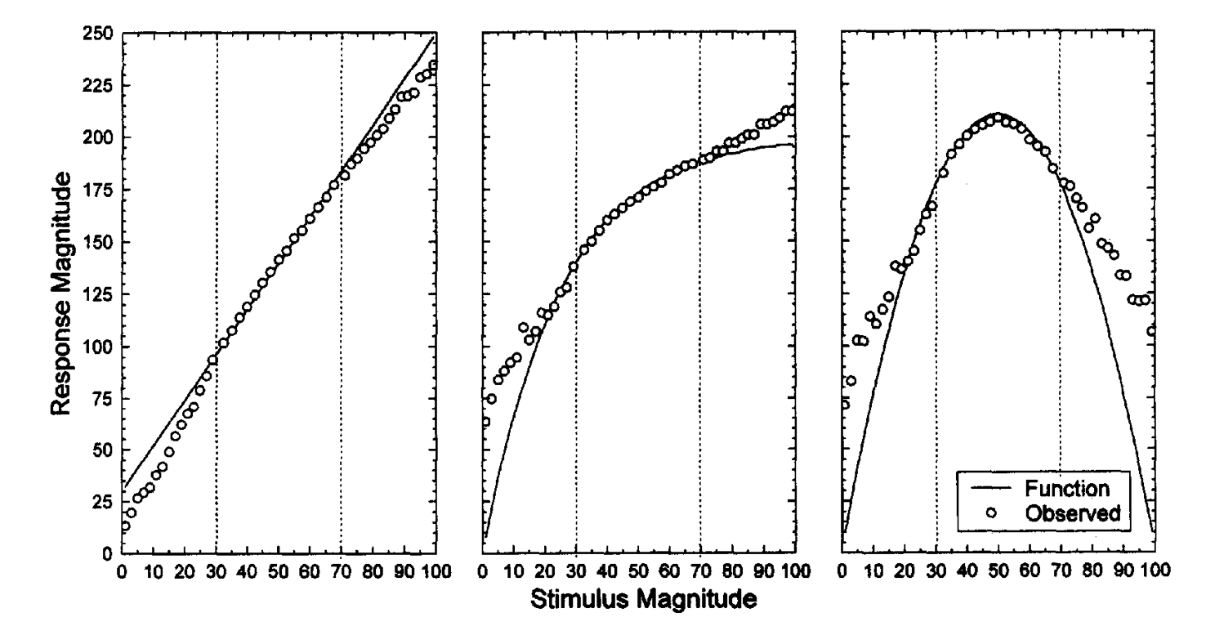
\includegraphics[scale=.4]{figures/delosh1997a.png}
    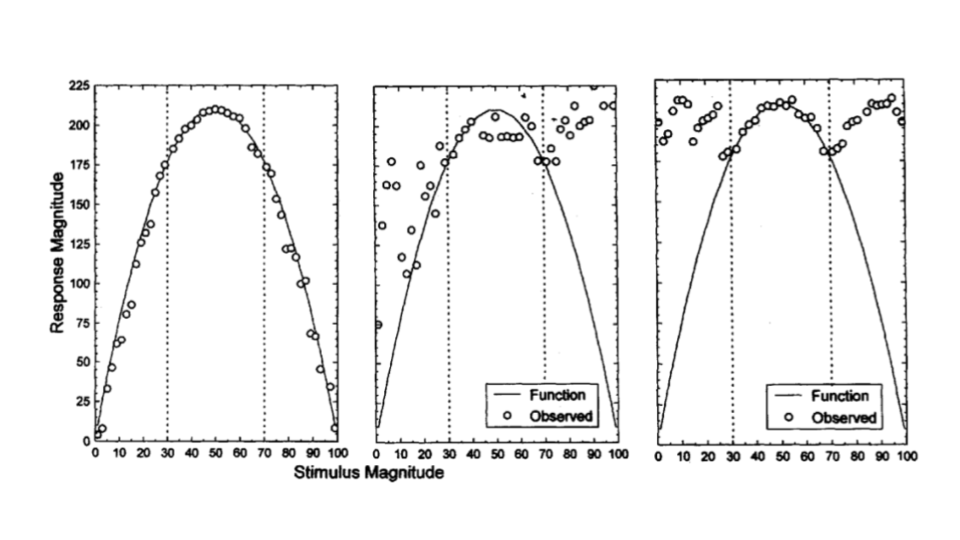
\includegraphics[scale=.5]{figures/delosh1997b.png}
    \caption{\textbf{Top}: Some of the mean extrapolation data from \textcite{delosh1997extrapolation}. Notice that the interpolation region is generalized much more accurately than the extrapolation region. \textbf{Bottom}: Examples of extrapolation data from 3 different subjects from the quadratic condition: one who learned the function almost perfectly, another that seemed to learn something akin to a linear function, and another who seemed to learn nothing at all. Taken directly from \textcite{delosh1997extrapolation}.}
    \label{fig:delosh1997}
\end{figure} 


\subsubsection{Models of Function Learning}
Early models of function learning (referred to in the FL literature as ``rule-based'') were analogous to statistical regression, assuming that psychological representations consisted of compositional basis functions that were tuned or selected for during learning (\cite{brehmer1974hypotheses,koh1991function}). For example, \textcite{brehmer1974hypotheses} found that interpolation behavioral data for a power, log, and linear function was best fit by a polynomial regression model biased towards power functions (relative to other regression models or associative stimulus-generalization models). While useful for predicting interpolation data, \textcite{delosh1997extrapolation}'s findings that humans often fail to extrapolate functional knowledge in a way that's consistent with the basis function presents a serious challenge for regression-based theories\endnote{An interesting alternative to early, regression-based models might be the autoencoder, which utilizes multiple layers of simple, linear-like functions to produce any particular nonlinear response (importantly, optimized via error-driven learning in a manner consistent with the typical training experience of human learners).}. 

The phenomena that humans extrapolate functional knowledge in a manner \emph{close-to-consistent} with the basis function also presents a serious problem for stimulus-generalization based theories (referred to in the FL literature as ``associative''). Inspired by the success of exemplar models in category learning (\cite{kruschke1992alcove}), associative models (\cite{delosh1997extrapolation,busemeyer1997learning}) assume that subjects retain a record in memory with the value of each presented cue during training; when encountering a new cue, subjects simply generalize the criterion value that was associated with similar cues in memory. An immediate problem with associative models is dealing with the phenomena that humans can interpolate to new items with accuracy indistinguishable from original training items (\cite{carroll1963functional,delosh1997extrapolation,koh1991function}). This consequently led \cite{delosh1997extrapolation} to propose a modification to their original ALM (associative learning model) that could linearly generalize from reference cues in memory when encountering new stimuli (referred to as EXAM\footnote{\textbf{EX}trapolating \textbf{A}ssociation \textbf{M}odel}). For example, if encountering a new cue between two previously observed cues, EXAM provides a mechanism for interpolating between the line that connects the two stimulus cues in memory\endnote{ALM and EXAM are implemented as associative, connectionist networks. One unusual property they share (relative to traditional connectionist networks) is the use of separate neurons for each discretized value of the stimulus dimension. For example, if coding for size ranging from 1mm to 10mm, ALM/EXAM might utilize 10 input neurons for each incrementing value. In more typical neural network (\cite{kruschke1992alcove,gluck1988conditioning,kurtz2007divergent}), only a single neuron is required to represent an entire stimulus scale. It's an open question whether ALM/EXAM's representational format is needed to accomplish the same theoretical predictions.}. In the case of extrapolation, (to the present author's understanding), EXAM extrapolates along the line connecting the largest or smallest set of training cues in memory\footnote{depending on whether extrapolation is in the smaller or larger direction}. \textcite{delosh1997extrapolation} found that the EXAM modification provided relatively excellent fits to human interpolation and extrapolation data (though the modification itself seemed to lack \emph{a priori} theoretical motivation).

Not long after, EXAM's explanatory success was challenged by a counter-intuitive phenomena prevalent in both the FL and CL literature: knowledge partitioning (\cite{yang2003context,lewandowsky2000knowledge}). Knowledge partitioning is a phenomena where subjects simultaneously generalize conflicting knowledge representations to a stimulus domain, often computationally explained via mixture-of-experts models (\cite{jacobs1991adaptive,erickson1998rules,kalish2004population}). For example, \textcite{kalish2004population} trained subjects on a function structure where most of the training cues followed a positive linear function --- with the exception of a few training cues that violated the underlying basis function. \textcite{kalish2004population} replicated \& extended a very counterintuitive, interesting phenomena\footnote{originally discovered by \cite{lewandowsky2000knowledge}} where some subjects simultaneously generalized both a positive and negative function during the test phase (see figure \ref{fig:knowledgePartitionStruct}). \textcite{kalish2004population} took their findings as evidence that a single subject can maintain multiple function representations within the same context, and found that their mixture of linear experts model (POLE\footnote{\textbf{P}opulation \textbf{O}f \textbf{L}inear \textbf{E}xperts}) was able to account for the phenomenon\footnote{\cite{yang2003context} further demonstrate that a mixture of experts model (ATRIUM; \cite{erickson1998rules}) can account for knowledge partitioning effects in the context of a category learning experiment.}. \textcite{kalish2004population} further demonstrate that \textcite{delosh1997extrapolation}'s EXAM model was unable to account for the knowledge partitioning finding (though see \cite{mcdaniel2009predicting} for a follow-up comparative study suggesting potential explanatory weaknesses in the POLE account)\endnote{Notably, mixture-of-experts models are somewhat agnostic to what the actual `experts' actually are. The knowledge partitioning phenomena doesn't necessarily contradict existing frameworks on it's own; rather, it can be taken as a theoretical argument about the role that contextual gating should play in computational models of category and function learning (similar to how dimensional attention has become an almost ubiquitous property of models of category learning; \cite{kruschke1992alcove,love2004sustain,erickson1998rules,waldron2001effects}).}. 

% POLE FIGURE 
\begin{figure}[H]
    \centering
    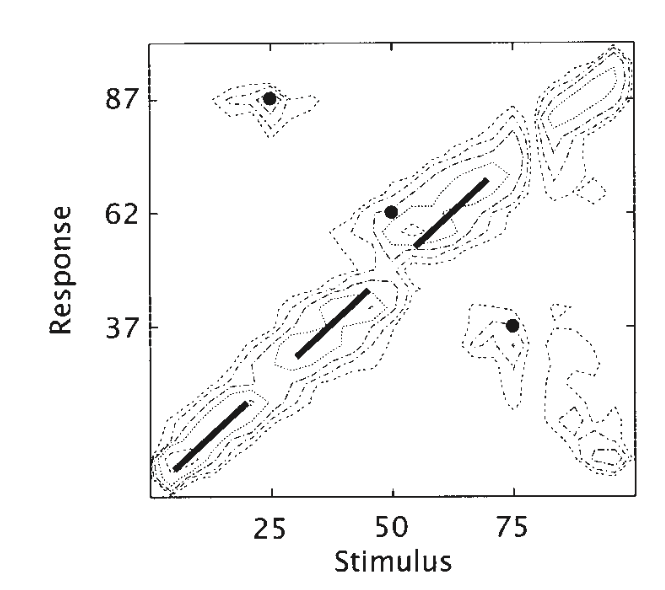
\includegraphics[scale=.4]{figures/knowledgePartitionStruct.png}
    \caption{Example of the function structure from \textcite{kalish2004population} that elicited knowledge partitioning effects. Taken directly from \textcite{kalish2004population}.}
    \label{fig:knowledgePartitionStruct}
\end{figure} 

The debate between associative and `rule-based' models appears unresolved\footnote{arguably, much like the debate between rule-based and similarity-based models of categorization}. While EXAM's success can be taken as support for associative models, it explicitly relies on a representation of linear functions when making interpolation and extrapolation decisions --- which seems like evidence partially supporting `rule-based' theories. Additionally, while not an empirically backed argument, the requirement of storing each exemplar during an FL experiment seems unnecessarily expensive (computationally), particularly when a single layer connectionist network --- i.e., regression --- can learn a linear function with 2 parameters (slope and intercept). In addition to existing accounts, Bayesian modeling is another more recent approach that is experiencing some preliminary success in the FL literature (\cite{lucas2015rational,narain2014structure,wu2020inference}). Given the fundamental importance of function learning in human cognition, theoretical explanations of how humans acquire and generalize functional knowledge will likely be a continuing research challenge for psychologists and computational theorists. Crucial next steps might lie in exploring function learning in the context of other cognitive domains (such as perceptual motor learning; \cite{rosenbaum2001acquisition}), or by learning functional relationships from raw perceptual data (as is currently being done in the categorization literature; \cite{singh2020end}).

% it'd be cool if you could have some simulation results from an MLP that does a much better job than all these models
	% ^ maybe a recurrent MLP that stores a record of the last n items in memory (maybe weighting the newest ones more)

\mbox{}\\
The next section will provide a similar (albeit briefer) review of the category learning literature, followed by a discussion of potential overlapping phenomena in both CL and FL research.

\subsection{Category Learning}

Category learning and understanding is a relatively broad field of research. Categories can range from being very simple and easy to describe with rules (e.g., things that are red), naturalistic and difficult to describe with rules (e.g., a bird), or structurally complex and abstract (the concept of evolution\footnote{Though, as will be argued in a later section, structurally complex `categories' might be better thought of as graphs of variables connected by both functional and categorical mappings}). While there are many ways through which category learning can be studied, computational theories of category learning have often relied on a very specific paradigm --- referred to as traditional, artificial classification learning (TACL; \cite{kurtz2015human}). 

The structure of a TACL experiment is almost identical to that of a function learning experiment: participants are shown a stimulus --- typically one at a time --- and asked to make a guess about the category membership of that particular exemplar. Subjects learn via corrective feedback provided after their guess. Similar to a function learning experiment, the training phase is typically followed by a generalization phase, where subjects generalize their categorical knowledge to novel, unseen stimuli\footnote{Typically, category learning studies don't distinguish between interpolation and extrapolation, since exemplars aren't typically sampled from a continuous function. However, the same general idea applies: generalization stimuli can lie inside or outside the range of items observed during training.}. Importantly, the past few decades of research have elucidated how human categorization behavior is sensitive to the particular nuances of an experimental procedure, such as category structure (\cite{shepard1961learning,kruschke1993human,nosofsky1992investigations,ashby1988decision}), curricula of stimulus exposure (\cite{kurtz1953effect,kornell2008learning}), learning objective (\cite{chin2004diagnosticity,kattner2016transfer}), and instructions \& context (\cite{kurtz2013human}). While a TACL experiment is a somewhat limited model of what real-world category learning is actually like, it has provided a number of interesting insights into the constraints learners face when trying to map observable stimulus features onto discrete labels.

Like the FL literature, the CL literature relies on a number of core phenomena that serve as benchmarks for computational explanations of categorization. One common benchmark comes from \textcite{shepard1961learning}, who trained subjects to map 3 binary-valued predictors (i.e., features) to a binary category label\footnote{2 possible categories}; specifically, \textcite{shepard1961learning} explored 6 different kinds of mappings between stimulus values and labels (figure \ref{fig:categoryStructs}, top). Importantly, \textcite{shepard1961learning} found a well-replicated disparity between the ease in which certain category structures were learned (\cite{nosofsky1994comparing}). One notable finding was that the easiest category structure to learn (by far) was the category structure that only required attention 1 stimulus feature (i.e., unidimensional\endnote{Some researchers have conjectured that an ideal category structure should efficiently maximize within-category similarity and minimize between-category dissimilarity (\cite{medin1987family}); the unidimensional preferences seems to be at odds with that conjecture.}); see \textcite{kruschke1993human} for a similar demonstration\footnote{\textcite{ashby2005human} describe these two structures (figure \ref{fig:categoryStructs}, bottom) as encompassing 2 different types of category learning problems: rule-based (left) and information-integration (right).} (figure \ref{fig:categoryStructs}, bottom). TACL experiments typically leverage stimuli with a small number of manipulatable features (2-5)\footnote{This contrasts with function learning studies, which typically only map one cued feature to one criterion feature.} --- which arguably deviates from most naturalistic, perceptual categories. Nevertheless, the literature has generally supported the idea that the challenge of mapping abstract, artificial variables in a laboratory setting gets harder as the number of required predictor cues increases. 

% figure: shj types and filtration
\begin{figure}[H]
    \centering
    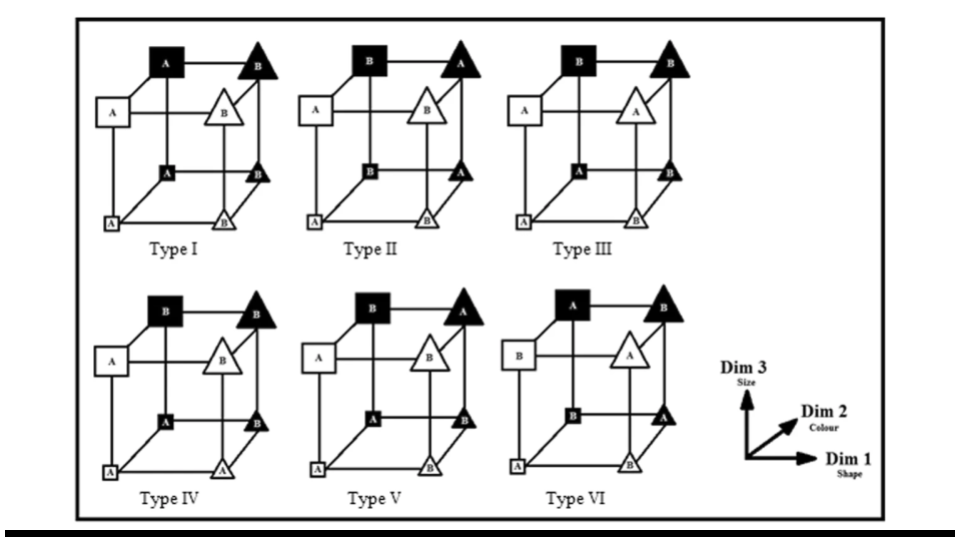
\includegraphics[scale=.4]{figures/shj6.png}
    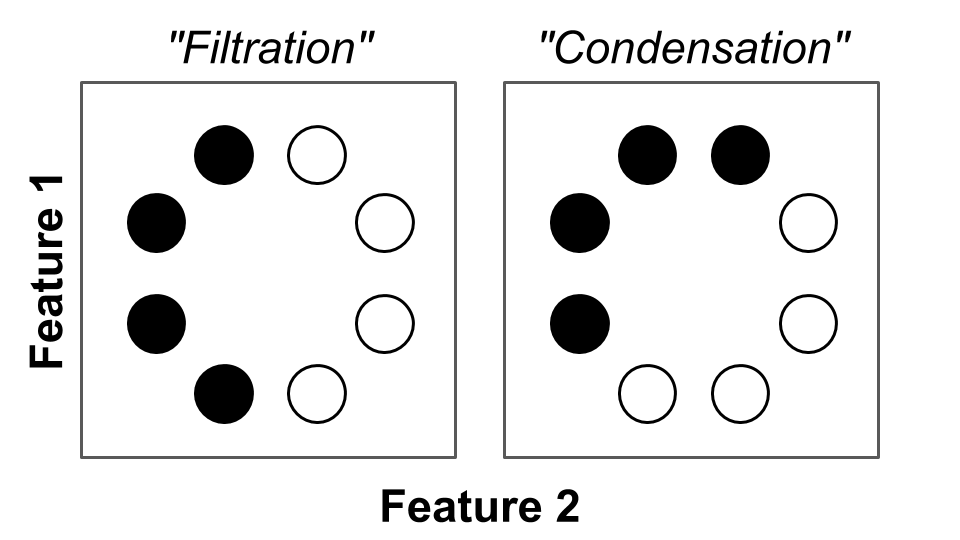
\includegraphics[scale=.4]{figures/krushke1993.png}
    \caption{\textbf{Top}: Visualization of the 6 different category structures from \textcite{shepard1961learning} in an arbitrary stimulus domain. Taken directly from \textcite{morgan2020comparing}. \textbf{Bottom}: Visualization of the `filtration' and `condensation' category structures used by \textcite{kruschke1993human}, who found that humans learned the filtration condition (which can be classified on the basis of \emph{a single} feature) easier to learn. Adapted from \textcite{kruschke1993human}.} 
    \label{fig:categoryStructs}
\end{figure} 

Predictions about which categories are easier to learn can also be a liability for some theories. For example, prototype theories predict that multidimensional categories should be easier to learn when they are linearly separable (i.e., can be separated by a multidimensional plane in the stimulus space); in constrast with this prediction, \textcite{medin1981linear} found that nonlinearly separable categories were as easy for subjects to learn as linearly separable categories\footnote{using stimuli defined by binary features}. Beyond the issue of ease of learning, another key phenomenon in the CL literature is the Categorical Perception effect (\cite{goldstone1994role,livingston1998categorical,pothos2014fickle}). In one demonstration, \textcite{goldstone1994role} queried subjects ability to perceptually discriminate between various stimulus pairs utilized in a TACL experiment. Critically, \textcite{goldstone1994role} found that subjects were much better at distinguished stimuli (post-learning) when those stimuli varied along diagnostic category boundaries (see \cite{goldstone2001altering} for a replication with similarity ratings)\footnote{Categorical perception effects provide an interesting benchmark for computational models, given that the phenomenon was popularized in the CL literature \emph{after} the formulation of many leading classic theories; meaning, any theoretical explanation of category perception effects would have to result from an \emph{a priori} prediction. In other words: classic theorists couldn't cheat).}.

\mbox{}\\
This section by no means covers the full variety of phenomenological effects uncovered by the TACL paradigm (though more will be discussed in a later section). Further, the TACL paradigm itself only encompasses a small scope of findings from category and concept learning literature as a whole (see \cite{murphy2004big} for a more thorough review). The next section will provide a brief (and again, incomplete) review of classic models of category learning (with a focus on those that inspired computational modeling in the FL literature).

\subsubsection{Models of Category Learning}

In the FL literature, models are typically described as falling into two camps: rule-based (curve fitting \& regression) and associative (stimulus generalization). The CL literature contains a similar division between models that leverage either logical rules (\cite{levine1975cognitive,nosofsky1994rule}), similarity to data-driven category representations (\cite{nosofsky1986attention,minda2001prototypes,love2004sustain,kurtz2007divergent}), or both (\cite{erickson1998rules}). Like models of FL, connectionism has been a fundamental framework for mediating different computational theories of categorization (\cite{gluck1988conditioning,kruschke1992alcove,kurtz2007divergent,erickson1998rules}). Associative and data-driven models of FL and CL also share the property of being implemented as a feed-forward, directed mapping between stimulus cues and responses. 

Bayesian cognitive modeling is another, implementation-agnostic, cross-domain framework that is gaining popularity in both the CL and FL literatures (\cite{anderson1991adaptive,sanborn2006more,griffiths2008categorization}). The Bayesian, or `rational' approach to categorization assumes that learners' objective during a CL scenario is to maximize the probability of successfully inferring the properties of novel objects using whatever representational mechanisms are available (\cite{griffiths2008categorization}). While classic theorists spent a great deal of effort debating the true nature of category representations in the human mind --- such as exemplar-based representations (\cite{nosofsky1986attention}), prototype-based representations (\cite{minda2001prototypes}), or something in between (\cite{love2004sustain,rosseel2002mixture,vanpaemel2005varying}) ---, Bayesian theorists assume learners are endowed with the mechanism to produce any arbitrary representational model that optimally captures the available data. Importantly, Bayesian theories don't necessarily conflict with existing frameworks, and can be fluidly integrated into other, more process-centric accounts (like connectionist models; \cite{neal2012bayesian}).

% - - - - - - - - - - - - - - - - - - - - - - - - - - - - - - - - - - - - - - - - -

\section{Key Areas of Present and Potential Overlap}

Computational explanations in both the CL and FL literatures share key elemental principles: (a) both rely on error-driven, trial-wise learning, (b) both constrain learning environment to a small number of easy-to-identify latent variables (serving as cues, features, response, and category labels), and (c) both rely on the same theoretical frameworks for designing computational models. The obvious difference is that the mappings between predictor and response variables are continuous in FL and discrete in CL. Another methodological difference is that FL studies often involve a single predictor variable, where as the stimuli in CL experiments contain multiple predictive features. Further, the predictor and response variables in FL studies are usually described as \emph{attributes} or \emph{properties} (such as weight, size, test scores, etc.); in contrast, the response variables in CL studies are typically framed as conceptual entities\footnote{This aspect alone could invoke different forms of prior knowledge; in other words, learners might enter a CL or FL study with the expectation that feature-to-feature mappings in the environment are typically described by continuous functions, while feature-to-entity mappings are typically described by discrete probability density functions (\cite{ashby1995categorization})}. One perspective is that the differences between CL and FL studies are largely in regards to methodological nuances, and both might evoke the same cognitive processes. This section will explore this perspective further to try to address the question of whether CL and FL rely on common mechanistic principles.

\subsection{Prior Knowledge}

One possible phenomenological overlap between CL and FL is the impact of prior knowledge. In the CL literature, a variety of studies have demonstrated the impact of prior knowledge during category learning experiments. One demonstration comes from \textcite{wattenmaker1986linear}, who found that subjects were better at learning linearly separable (relative to nonlinearly separable) categories only when stimulus features shared a common underlying theme (e.g., all related to the feature of ``being honest''). The opposite effect emerged when features where framed as being independent\footnote{\textcite{wattenmaker1986linear} used abstract descriptions of stimuli rather than stimuli defined by perceptual characteristics, which may be pertinent to the generalizability of their findings.}. In another demonstration, \textcite{heit1994models} found that subjects were better at inferring relations between discretely-valued features when the feature relationships were congruent with prior knowledge\footnote{For example, pairing the feature \emph{shy} with the feature \emph{avoiding parties} would be congruent with prior knowledge, while pairing the feature \emph{shy} with \emph{attends parties} would be at odds with prior knowledge.}. In a very similar preparation, \textcite{heit1995belief} found that that same effect of prior knowledge slowly diminished as learning progressed; that is, subjects eventually updated their knowledge to match the unintuitive feature relationship defined in the experiment (similar to a finding in the FL literature from work by \cite{sniezek1986role}). 

While not particularly surprising, subjects in both FL and CL experiments appear to leverage prior biases about how functional and categorical variables interact\footnote{In fact, this particular bias of prior knowledge is often explicitly guarded against when designing experiments (\cite{kurtz2015human}).}. Further, subjects are eventually able to update their prior beliefs in response to experimental feedback. This common phenomenon doesn't necessarily suggest a mechanistic overlap between CL and FL in humans; however, it does have implications for CL and FL theories. Speculatively, the representations underlying human CL and FL may be driven by the nature of prior experience in everyday environments rather than the nature of cognitive mechanisms entirely\footnote{Which partially aligns with arguments made by Bayesian theorists (\cite{anderson1991adaptive,griffiths2008categorization})}. However, to the author's knowledge, there doesn't appear to be any systematic investigation of the nature of functional and categorical relationships between psychologically-relevant variables in ecologically representative environments\endnote{Though \textcite{rosch1975family} argue that \emph{family resemblance} is a particularly common property of naturalistic categories; interestingly, however, \emph{family resemblance} structures seem to lack any particular bias in artificial, low-dimensional stimulus domains (\cite{shepard1961learning,medin1987family}).}.

\subsection{Inference Learning}

In a standard TACL experiment, subjects are given a set of stimulus features, and asked to decide which category it belongs to. An alternative learning objective --- known as \emph{inference learning} (\cite{yamauchi1998category,chin2004diagnosticity}) --- directs subjects to try and guess the value of a stimulus feature \emph{given} a presented category label (as well as the rest of the stimulus features). Rather than mapping stimulus features to category labels, subjects are guided to focus on the within-category statistical relationships between features (see \cite{kurtz2007divergent} for an example of a connectionist model that learns in a similar way). \cite{chin2004diagnosticity} found that inference learning had important implications on what subjects learned stimulus exposure: inference learners were more sensitive\footnote{Sensitivity to stimulus features was measured via a classification task using stimuli with partially occluded features.} to \emph{prototypical features}, whereas classification learners were more sensitive to \emph{diagnostic features}\footnote{Prototypical features are features shared by the majority of category exemplars; diagnostic features are features that help differentiate category labels. Both are orthogonal but neither are mutually exclusive.} (see \cite{yamauchi1998category} for an earlier demonstration of this phenomenon). Inference learning is a particularly interesting learning objective given that it is essentially the same as a function learning objective, except (1) there is the presence of a discrete cue (the category label), (2) feature values are typically binary instead of continuous (though there's no reason why they need to be\footnote{\textcite{ell2020learning} seem to be the only example of an inference learning objective on continuously valued features in the CL literature.}), and (3) a single feature often alternates between being a \emph{predictor} or a \emph{predicted} cue\footnote{Relatedly, \textcite{surber1987formal} found that subjects trained to map feature 1 $\rightarrow$ 2 \emph{do not} consequently learn the inverse mapping between feature 2 $\rightarrow$ feature 1}. 

The key finding from the inference learning literature is that the nature of category representations are influenced by the objective subjects are trying to solve (\cite{yamauchi1998category,chin2004diagnosticity,ell2020learning}). The inference learning literature also demonstrates how category learning and function learning can be fluidly integrated into the same experimental preparation. Further, subjects ability to seamlessly integrate both \emph{feature}$\rightarrow$\emph{category} and \emph{feature}$\rightarrow$\emph{feature} mappings in the same context highlights an innate predisposition to do so. One (more cautious) interpretation might conclude that the mechanisms that underlie category and function learning in humans are designed to interact. Another (more extreme) interpretation is that the underlying mechanism of CL and FL are identical --- the only key difference being \emph{distributional properties of} and \emph{statistical relationships between} latent variables as they typically occur in a learner's naturalistic environment. This extreme interpretation will be explored further in a later section (\ref{sigmoid_section}).

\subsection{Dimensionality}

\textcite{shepard1961learning}'s and \textcite{kruschke1993human}'s demonstrations highlight the phenomenon where learning is more difficult as the number of relevant dimensions increase. This might seem unsurprising, but it highlights an explanatory limitation for traditional neural network models of cognition (which don't seem sensitive to sparsity of predictive features); \cite{kruschke1993human}). \textcite{kruschke1993human} took this as evidence of a selective attention mechanism in human categorization. While there is no direct analog in the FL literature (see \ref{fl_k93} for a proposal), there is a number of empirical demonstrations that show humans are sensitive to dimensionality (or, number of predictive cues) in a function learning experiment. One such example is the \emph{cue competition effect}, where subjects have difficulty integrating the combined predictability of 2 cues when one cue is more predictive than the other (\cite{busemeyer1993cue}; see \cite{kruschke1999model} for a review of cue competition effects in the probabilistic category learning literature). 

The cue competition effect seems counterintuitive, given that the statistically optimal thing to do in a \emph{multiple cue probability learning} experiment is to integrate as many predictive features as possible. However, humans in both CL and FL preparations seem to selectively weight various features, even when those features are statistically correlated (\cite{gluck1988conditioning}). One explanation might be that the mechanisms for forming functional and categorical mappings between latent variables are cognitively demanding, and that there is an implicit bias to reduce the dimensionality of the learning domain --- thereby freeing up computational resources. A more specific explanation is provided by \textcite{kruschke1999model}, who argued that attentional biases in cue learning are optimal for forming useful representations from a relatively limited number of case exposures. Another alternative (but not mutually exclusive) explanation --- which will be discussed in more detail later (\ref{graphs}) --- is that CL and FL in humans is subsumed by a larger computational challenge of global knowledge organization. Specifically, if the goal of FL and CL is to form predictive mappings between latent variables contained within a large-scale knowledge graph, than the computational efficiency of navigating that graph might benefit from a bias towards sparse connectivity.

\subsection{Future Directions for Comparative Investigations}

The next section will describe findings from the CL literature that (to the author's knowledge) have yet to be applied to the FL literature, but might help address the question of whether FL and CL share overlapping mechanisms.

\paragraph{Formal Metrics of Function Learning}\mbox{}\\

Computational process models of FL and CL provide mechanistic explanations of why some data are easier / harder to learn than others. An additional branch of theoretical categorization research aims to formally describe why some category structures are more difficult to learn than others --- independent of whatever computational processes are trying to learn them (\cite{pape2015complexity}). For example, \textcite{feldman2000minimization} found that the ease of learning the six category structures from \textcite{shepard1961learning} was correlated with the boolean complexity of each structure (that is, the simplest boolean circuit that can map a set of binary features to a binary category label). An alternative demonstration comes from \textcite{pape2015complexity}, who found that the ordering of learning difficulty was predictive by the information complexity of each structure. While formal metrics don't necessarily provide mechanistic explanations of category learning, they do help elucidate either the \emph{information subjects are sensitive} to or the \emph{learning objective they are trying to solve}.

To the author's knowledge, there aren't any formal metrics of why some functions might be easier to learn than others. However, providing a formal metric to explain function learning difficulty fundamentally contrasts from ongoing efforts in the CL literature --- particularly when the stimulus features and category labels are typically assumed to be binary. A formal analysis of function learning might require an analysis of the mathematical or information-theoretic properties of continuous function families, which is far beyond the scope of this paper\footnote{and this author's ability to do so}. However, a potential formal metric could build on some of the assumptions made by existing process models, such as compositionality (\cite{schulz2017compositional}). For example, \textcite{kalish2004population}'s POLE model of function learning assumes that subjects represent functional knowledge via a piecemeal of composite, linear functions. If this assumption is accurate, the difficulty of learning certain functions over others might be formalized as the number of linear functions required to adequately minimize predictive error during generalization --- in which case, the comparative difficulties in learning various function families (linear, quadratic, exponential, periodic) start to become a bit more intuitive. However, that metric specifically would still leave many questions unanswered, such as the preference of positive linear functions (relative to negative linear functions; \cite{naylor1968intuitive,brehmer1974hypotheses}).

\paragraph{Representational Shifts in FL}\mbox{}\\

As discussed earlier, \emph{categorical perception} is the relatively well-replicated phenomena where learner's perceptual descriptions of a stimulus domain shift after exposure to a category learning preparation (\cite{goldstone1994role,liberman1957discrimination,harnad1987psychophysical,livingston1998categorical}). For instance, \textcite{goldstone1994role} found evidence that TACL-style classification learning improved subjects' ability to discriminate between stimuli that varied along diagnostic boundaries (figure \ref{fig:CPinFL}a). Further, categorical perception effects are often dichotomized into 2 distinct phenomena: between-category \emph{expansion} (where stimuli from opposing categories are viewed as more dissimilar; easier to distinguish) and within-category \emph{compression} (stimuli from the same category are viewed as more similar; harder to distinguish). The specific directions of representational shifts (like compression and expansion) might reflect the nature of category representations subjects acquire during learning.

While it's hard to confidently infer what subjects are actually perceiving during an experiment\footnote{Typically, perceptual changes are measured via stimulus discrimination accuracy or pairwise similarity ratings; whether this tightly corresponds to conscious perception is an open question.}, the idea that the perceptual system can align itself to the conceptual demands of the learner is a fascinating theoretical concern. To the author's knowledge, categorical perception effects have not been explored using inference learning or function learning preparations\footnote{Though if they were, the phenomenon would probably require a different name.}. Given that regression-style (or, `rule-based') theories assume that functional knowledge is represented via basis functions, it seems relatively plausible that perceptual changes (measured via stimulus ratings or discriminability tasks) might occur towards the underlying basis function being learned (figure \ref{fig:CPinFL}b). 

\begin{figure}[H]
    \centering
    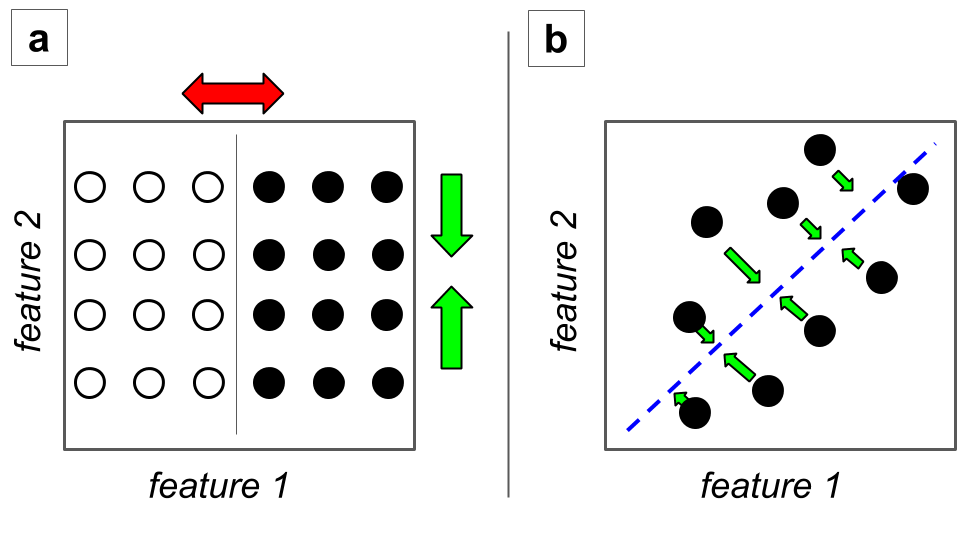
\includegraphics[scale=.4]{figures/CPinFL.png}
    \caption{\textbf{a}: Example of the category structure used by \textcite{goldstone1994role}; red arrows indicate \emph{expansion} effects, green arrows indicate \textbf{compression} effects. \textbf{b}: Visualization of the direction of compression effects one might expect in a function learning task.}
    \label{fig:CPinFL}
\end{figure} 

\paragraph{FL Replication of \textcite{kruschke1993human}} \label{fl_k93} \mbox{}\\

In a relatively impactful demonstration, \textcite{kruschke1993human} tested learning of 2 category structures, labeled `\emph{filtration}' and `\emph{condensation}' (figure \ref{fig:categoryStructs}, bottom). Importantly, the stimulus coordinates (or, feature values) in both category structures were identical; the only difference is that in one structure (\emph{filtration}), only 1 stimulus feature was needed to correctly classify each exemplar. In the other structure (\emph{condensation}), each feature was partially predictive of category membership. \textcite{kruschke1993human} found that the \emph{filtration} structure was learned faster than the \emph{condensation} structure, which \textcite{kruschke1993human} argued was evidence for selective attention in CL. To the author's knowledge, no similar demonstration has been made using an analogous pair of function structures --- though such a demonstration might be relatively straightforward to produce. For example, one could train subjects on a 3 dimensional linear manifold; in one case, only 1 feature is needed to accurately predict the criterion value (figure \ref{fig:filt-cond-func}a), while in the other case, both features are jointly predictive of the criterion value (\ref{fig:filt-cond-func}b). If the mechanisms of CL and FL overlap, then one might expect a similar advantage of learning functional patterns that require fewer relevant cues.

% figure of filtration/condesnation in both krushkes version and FL version im making up
\begin{figure}[H]
    \centering
    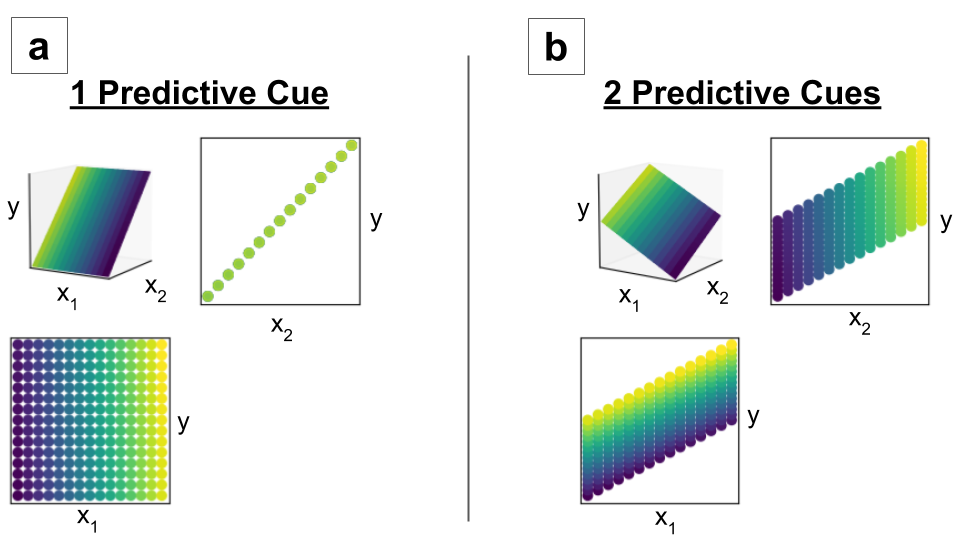
\includegraphics[scale=.4]{figures/filt-cond-func.png}
    \caption{Example of a function learning problem involving 2 continuous predictive cues and 1 continuous criterion. In the first structure (a), only one feature is needed to perfectly predict the criterion (y-axis). In the other (b), both features are needed to predict the criterion. Color indicates a unique identifier for each stimulus coordinate. 3D plots show relationship between all 3 variables; 2D plots show the isolated relationships between each cue $X_1$, $X_2$ and the criterion value $Y$.}
    \label{fig:filt-cond-func}
\end{figure} 

% - - - - - - - - - - - - - - - - - - - - - - - - - - - - - - - - - - - - - - - - -

\section{Further Discussion}

\subsection{Flexibility of Monotonic Functions}\label{sigmoid_section}

Connectionism (\cite{rumelhart1986general}) has been a core framework for psychological theories across a variety of domains within psychology, including (but no limited to) categorization (\cite{kruschke1992alcove,kurtz2007divergent,gluck1988conditioning}), function learning (\cite{kalish2004population,delosh1997extrapolation}), analogical reasoning (\cite{tomlinson2006learning}), and semantic understanding (\cite{rogers2004semantic}). However, the connectionist framework itself is actually relatively "theory-agnostic", in that it can be used to instantiate completely divergent theoretical explanations of a psychological construct\footnote{In the case of categorization, for example, connectionist models have been used to instantiate models of both exemplar (\cite{kruschke1992alcove}) and prototype theories (\cite{johansen2002there}).}. Rather, connectionism provides a computational framework for which theories can be instantiated in a brain-style system.

To reiterate, while many leading models of category learning and function learning leverage the connectionist framework (\cite{kruschke1992alcove,kurtz2007divergent,delosh1997extrapolation,kalish2004population}), they often make very distinct fundamental predictions. As a result, the fact that leading theoretical models rely on connectionism doesn't necessarily provide a cross-domain computational explanation of CL and FL in humans. Interestingly, an activation function commonly used by connectionist models --- the sigmoid function (figure \ref{fig:sigmoid}) --- is adequately equipped to handle both categorical and functional mappings (and even capable of approximating the radial basis function used by exemplar models of categorization; \cite{nosofsky1986attention,kruschke1992alcove})\endnote{The sigmoid function might also be particularly useful because it can approximate an analog$\rightarrow$digital conversion (or vice versa), which might shift the computational complexity of certain problems (an idea discussed earlier by \cite{harnad1987psychophysical}).}. For categorical decisions, a sigmoid function can take the form of a binary decision boundary indicating the presence or absence of a category member given data from the environment (figure \ref{fig:sigmoid}a). For function learning, a sigmoid function can approximate linear relationships (figure \ref{fig:sigmoid}b); in a traditional multilayer neural net, a set of sigmoids can be aggregated to approximate more complex functions\footnote{similar (but distinct) from the approach taken by POLE (\cite{kalish2004population}, which piecemeals linear functions per specific datapoints rather than aggregating all functional representations it has access to)}. Critically, whether a network of sigmoid functions learns categorical or functional mappings depends on the \emph{data from the environment} it's presented with, bearing resemblance to a differentiable circuit that can approximate both logical operations \emph{and} functional associations.

\begin{figure}[H]
    \centering
    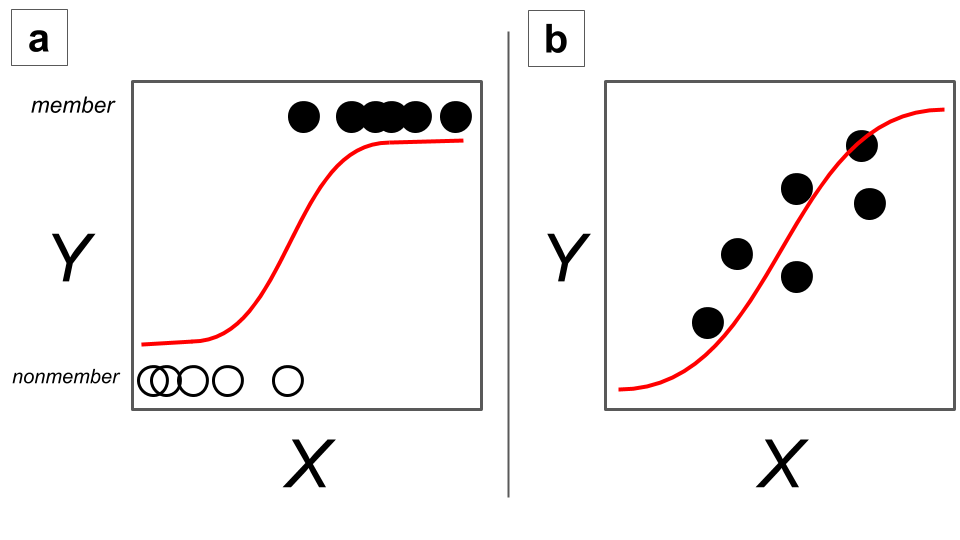
\includegraphics[scale=.4]{figures/sigmoid.png}
    \caption{Example of 2 distinct uses of the sigmoid function. \textbf{a}: A sigmoid function being used to form a probabilistic decision rule about the presence of a given category given a continuous predictor feature $X$. Note that the sigmoid function closely approximates the \href{https://en.wikipedia.org/wiki/Normal_distribution}{cumulative normal distribution}. \textbf{b}: The linear portion of a sigmoid function being used to approximate a linear relationship between continuous predictor $X$ and continuous outcome $Y$. When tuning a sigmoid function via gradient descent, the particular form of the function depends on the distribution of values within the predictor and outcome variables.}
    \label{fig:sigmoid}
\end{figure} 	

While a network of sigmoid neurons is adaptive enough to handle both classification and function learning problems, it's an open question whether this type of model is psychologically meaningful. In the CL literature, multilayer sigmoidal networks have provided poor fits to behavioral data (see \cite{kruschke1993human} for an analysis about why these failures arise). For example, \textcite{kruschke1993human} found that a sigmoidal network (trained via backpropagation) was unable to demonstrate the comparative differences humans exhibit when learning categories diagnosable by 1 or 2 relevant features\footnote{To reiterate, humans learned faster when the categories could be diagnosed on the basis of 1 feature}. However, this empirical failure was alleviated when \textcite{kruschke1993human} included attentional weights in the input layer of a standard sigmoidal network (in addition to fixing the weights of the sigmoidal neurons). Further, \textcite{kruschke1993human} highlighted that a sigmoidal neural net could approximate exemplar models by using a "place coding" scheme where input values are discretized and treated as individual features (similar to the approach taken by EXAM; \cite{busemeyer1997learning}). While there's been little work extending \textcite{kruschke1993human}'s sigmoid-based exemplar-approximation model to the rest of the CL literature, it never-the-less highlights the explanatory power of networks of strictly monotonic functions with a magnitude ceiling (i.e., the sigmoid).

% figure showing APPLECOVE or whatever

But what about function learning phenomena? The empirical failures of rule-based models at predicting extrapolation performance might suggest a preliminary weakness in a regression-style explanation of human function learning. However, previous rule-based models typically utilized relatively complex functions, such as polynomial or exponentials (\cite{brehmer1974hypotheses}). An alternative  approach --- \textcite{kalish2004population}'s POLE model --- uses a composition of strictly linear functions to explain FL in humans. While POLE can account for knowledge partitioning effects, it fails to account for a key extrapolation phenomenon from \textcite{mcdaniel2009predicting}. To the present author's knowledge, researchers haven't explored whether a composition of sigmoid functions (i.e., a standard, multilayer neural net with sigmoid activations) can explain transfer phenomena in human FL. Interestingly, the extrapolation data from \textcite{delosh1997extrapolation} and \textcite{mcdaniel2009predicting} (experiment 2) are relatively well predicted when fitting the training functions using a combination of 1-2 sigmoid functions (figure \ref{fig:sigFit}).

% say that im cheating
\begin{figure}[H]
    \centering
    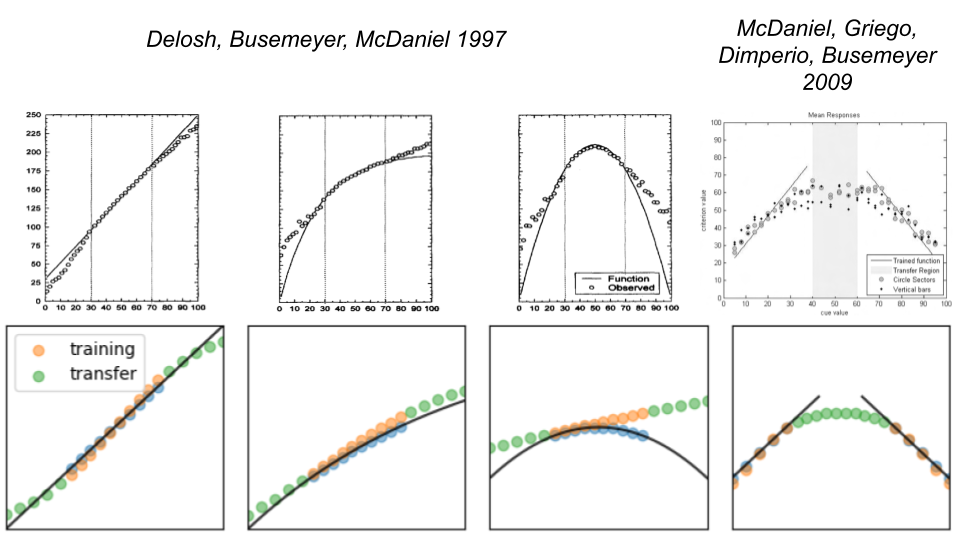
\includegraphics[scale=.4]{figures/sigFit.png}
    \caption{Example of a neural net with sigmoidal hidden units fit to \emph{transfer} data of \textcite{delosh1997extrapolation} and \textcite{mcdaniel2009predicting}. Top row shows experimental data from humans; bottom row shows neural net predictions. In each function structure, only 1 sigmoid hidden node was used (except for the last function from \textcite{mcdaniel2009predicting}, where 2 sigmoid nodes were fit to both linear training functions). Weights were tuned by the author (not through backpropagation), making this demonstration more of a proof-of-concept than a psychologically meaningful explanation.}
    \label{fig:sigFit}
\end{figure} 

A big limitation with the above analysis is that the sigmoid functions were fit post-hoc by the author (making it relatively easy to cheat); what's missing is an a priori system for learning the training data\footnote{The author found that backpropagation alone doesn't seem to be sufficient.}. In addition, these results aren't necessarily surprising given that neural networks are universal function approximators (given enough hidden neurons; \cite{csaji2001approximation}); this alone makes the present explanation unfalsifiable. However, penalizing the number of required sigmoid representations a learner requires might provide a more falsifiable explanation of the nature of extrapolation behavior as well as the comparative ease through which some functions are learned over others (by assuming that the difficulty of learning a functional relationship is correlated with the number of sigmoid functions needed to approximate it).

\textcite{kruschke1993human}'s demonstration that sigmoidal networks can approximate leading accounts of category learning --- in addition to the preliminary, rough demonstration by the present author regarding FL extrapolation with sigmoids --- provides some support for the argument that CL and FL overlap mechanistically. Specifically, the cognitive mechanism that underlies learning and generalization of both functional and categorical mappings between latent variables might be explained (in part) as a process of compositional, data-driven approximation using monotonic representations\endnote{Why might monotonic functions with a magnitude ceiling be useful for network-style learning? One possible explanation is in regard to mechanism through which representations are updated during learning. Assuming the mind is a network doing anything akin to backpropagation (see \cite{lillicrap2020backpropagation}), then the plasticity of neurons are influenced by the `loss landscape' (\cite{li2018visualizing}) defined by the network's optimization goal. Monotonic functions might be useful for producing smooth landscapes (with less local minima) that are easy for the network to traverse (relative to non-monotonic radial basis or periodic functions; \cite{parascandolo2016taming}).}. This doesn't, however, explain how humans can acquire verbalizable, algebraic knowledge defining the relationships between latent variables in the environment, which might indicate the necessity for a separate cognitive `system' (as argued by \cite{ashby1998neuropsychological}). Alternatively --- instead of a separate, distinct system --- the feedforward mappings formed through circuits of sigmoid functions might additionally interact with explicit, recurrent memory (which might also leverage sigmoid and \emph{sigmoid-like} functions; \cite{gers2001lstm})\footnote{See also \textcite{graves2014neural} for an example of an end-to-end, memory-augmented recurrent network that learns to perform explicit symbolic operations.}; this might alleviate the need for a dual-systems theoretical explanation\endnote{See also \textcite{tsukimoto2000extracting}'s method for approximating boolean functions from sigmoidal neural nets.}.


\subsection{Implications of Graphical Knowledge Representation} \label{graphs}

An important research question regarding the mechanisms of CL and FL in humans (whether those mechanisms are similar or distinct) is how both processes fit within the larger framework of human cognition as a whole. The majority of the categories and functions humans learn are not learned in the laboratory, and the inherent purpose of CL and FL probably isn't to improve accuracy during an experiment. Learning functional and categorical mappings between variables (which will be referred to as \emph{latent mappings} for the remainder of this section) is clearly useful for navigating through and predicting events in the environment; but, do these learned representations exist as isolated parcels of knowledge?, or are they components within a much larger, more complex representational system? If so, what might that representational system look like?

Graphs are a type of data structure that can be defined as a network of nodes (variables) connected by any type of relationship (\cite{newman2003structure}). In addition to being a recently emerging interest in the machine learning literature (\cite{wu2020inference,bronstein2017geometric,schlichtkrull2018modeling}), graphs have had a rich history in cognitive science. Graphs have also served as the fundamental data structure for early theories of semantic knowledge, dating back to the \emph{spreading activation} theory (\cite{quillian1967word,collins1969retrieval,collins1975spreading}). Graphs (more generally, \emph{network science}) have been and are beginning to be a central part of many psychological literatures, include: language (\cite{vitevitch2008can}) \& statistical learning (\cite{saffran1996word,lynn2019graph}), procedural motor learning (\cite{kahn2018network}), semantic memory (\cite{abbott2012human}), causal cognition (\cite{danks2014unifying}), and analogical reasoning (taking the form of propositional networks; \cite{gentner1983structure}) --- to name a few. When thinking about how CL and FL representations fit into the broader scheme of cognition, it seems that graphical representations are a worthwhile (but speculative) assumption to start with.

What implications would graphical representations have for theories of CL and FL\footnote{beyond \cite{danks2007theory} early, innovative demonstration that may theoretical models of category learning could be described as directed graphical models}? First, we can assume that the cues, category labels, and stimulus features used in a standard CL or FL procedure all invoke typical latent variables subjects' find meaningful and disparate (otherwise, they probably wouldn't work in an experiment). Then, we can hypothesize that a supervised training procedure in both FL and CL involves learning a probabilistic or rule-based mapping between those latent variables\footnote{Importantly, it doesn't necessarily matter whether these mappings are learned via multiple systems (\cite{ashby1998neuropsychological}), multiple representations (\cite{erickson1998rules,kalish2004population}), or via data-sensitive applications of a single type of monotonic function (as discussed in the previous section); making this conceptual framing somewhat theory-agnostic at the level of isolated mappings.}; whether the mappings learned are functional or categorical depends on (at least in part) the latent variables' distributions of values as well as the biases invoked during the context of the learning task. For example, during a category learning experiment, a subject might be told that a set of stimulus features `\emph{is a}' member of a given category (or, \emph{`belongs to' category \emph{X}})\footnote{In the case of function learning, the subjects might hear language like `\emph{How much?}' or `\emph{How Many?}'}. This language might immediately cue learners as to what type of latent mapping they should expect to observe. Individual differences in CL and FL studies might also be influenced by the types of mappings each subject has a history of observing (in addition to other variables like fatigue, stimulus presentation order, etc), or what latent variables get activated by the experiment context.

The literature discussed thus par in this paper has focused on a specific type of FL and CL learning procedure --- \emph{supervised learning} --- where subjects are explicitly told the correct values mapping cues / features to criterion variables / category labels. The premise of this section is to say that these operations (both supervised CL and FL) correspond to a specific type of graphical operation: \emph{edge learning}\footnote{where predictor and predicted variables are nodes, and the relations between them are edges}. However, supervised learning is not the only relevant process in CL and Fl. For instance, in an unsupervised category learning experiment\endnote{To the author's knowledge, there is no analogous, unsupervised preparation in the function learning literature. It's unclear what impact such a preparation would have on subjects' ability to learn functional relationships. Speculatively, the presence of functional relationships might predict what latent variables subjects find most important. For example, given an environment with a large set of potential variables of interest, variables that have an obvious relationship (either categorical or functional) might be especially relevant in the future --- in that they allow subjects to make predictions in situations where information is limited.} (\cite{pothos2011measuring}), subjects are not explicitly told which category an item belongs to. Rather, subjects are presented with stimuli and tasked with determining the category labels on their own (typically by sorting a set of stimuli into groups they find most intuitive; \cite{pothos2011measuring,medin1987family}). This type of learning experience seems quite distinct from supervised learning of latent variable mappings, and might be better described as a process of \emph{latent variable discovery}; that is, the generation of new nodes within a larger knowledge graph. The structural context that describes a subjects' history with latent variables in the environment might be a key explanatory variable in why certain category structures are intuitively preferred over others during unsupervised acquisition.

Beyond simply re-framing the problem, what theoretical advantages are gained by proposing graphical representations as a central data structure for both CL and FL? The paradigm through which CL and FL are investigated in the lab attempts to reduce the learning context down to a few isolated variables with the goal of invoking as little prior knowledge as possible (\cite{kurtz2015human}). However, if the goal of CL and FL research is explanatory generalizability, then it's important to focus on how the phenomena and principles that describe experimental data apply to real world knowledge. Given that many real world knowledge domains seem to embody network structure --- e.g., semantic knowledge (\cite{collins1969retrieval,steyvers2005large}), phoneme structure in the English language (\cite{vitevitch2008can}), causal knowledge (\cite{danks2014unifying}) --- then thinking about CL and FL as computational operations on a graph might help explain how people learn categorical and functional relationships in real-world domains. Additionally, graphical data structures provide valuable information for learning and inference at the \emph{level of individual variables}. For example, if my goal was to infer the attributes of \emph{person X}'s social media profile, then I might benefit from looking at the features and attributes of the people that \emph{person X} is connected to. The machine learning literature is currently demonstrating that graphical data structures are very useful for inference and classification of category exemplars (which are arguably the objectives of theoretical models of CL and FL); it therefor seems reasonable (but again, speculative) that the human mind might leverage graphical data structures as well.

To summarize, this section posits the idea that supervised CL and FL in humans both correspond to computational operations between latent variables in a larger graphical representation of knowledge. Unsupervised learning can then be thought of as \emph{graph construction} (\cite{wu2020comprehensive}), where new nodes are both added and mapped to existing nodes (or, cues / features). Making this theoretical assumption provides a medium through which CL and FL can be framed in the larger context of other cognitive literatures, and explains how humans can make inferences about their environment using information \emph{beyond} strictly the variables they are presented with (leveraging the graphical structure of the domain that is invoked). Graphical representations also provide a shared representational structure that might explain how knowledge is transferred across domains --- an assumption already leveraged heavily by theoretical models of analogical reasoning, which typically invoke \emph{propositional} graphs as a fundamental representational structure (\cite{gentner1983structure,hummel1996lisa}). An exciting new step for cognitive modeling might lie in recent advances in applying data driven approaches (like deep learning) to graph structured learning problems using the same connectionist principles that constrain many psychological models (\cite{wu2020comprehensive,schlichtkrull2018modeling}).

% some kind of figure of a knowledge graph
\begin{figure}[H]
    \centering
    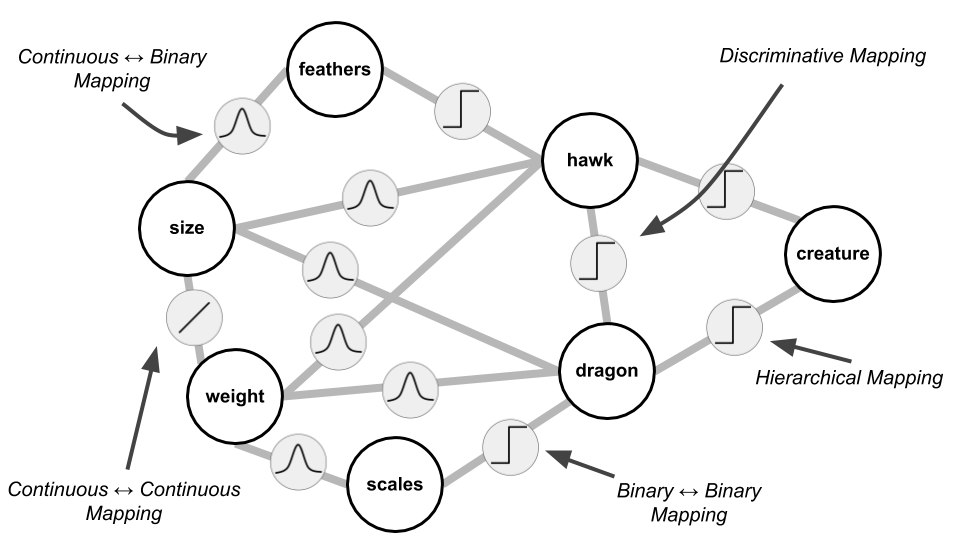
\includegraphics[scale=.4]{figures/knowledgeGraph.png}
    \caption{Example of a theoretical knowledge graph, where cues, features, and category labels are all treated as latent variables in a graph. The type of mapping between variables would be determined on each variable's distribution of values (as well contextual factors, experiment instructions, individual biases, etc). Note that these different types of mappings can all be approximated with a sigmoid function.}
    \label{fig:knowledgeGraph}
\end{figure}    

\subsection{Relationship to Other Branches of Cognitive Science}

It's beyond the scope (and ideal length) of this paper to provide an exhaustive review of how CL and FL in humans relates to other key branches of the psychological literature; this section will simply highlight a few attempts that have already been made. For instance, there have been a number of previous demonstrations highlighting the link between theories of categorization and theories of associative conditioning in animals (see \cite{kruschke2001toward,gluck1988conditioning}). The function learning literature does not seem to have been the subject of such an endeavor; however, it's close ties with the multiple cue probability learning literature suggests a link as well (\cite{kruschke1999model,busemeyer1997learning}). There has also been suggestions of an overlap between phenomena in FL literature and the procedural motor learning literature \cite{rosenbaum2001acquisition}). This link is a particularly interesting suggestion, given that it provides support for a speculative hypothesis that abstract intelligence might have evolved from --- or co-evolved with --- the original mechanisms for spatial navigation in complex physical terrains. In other words, the cognitive mechanism that allows a person to apply the correct amount pressure to the gas petal of a car\footnote{This example of a function learning task in the real-world was originally used by \cite{lucas2015rational}.} might be the same underlying mechanisms that allows a person to understand the relationship between energy use and monetary expense (the fundamental difference being whether the latent variables are perceptual or symbolic).

\subsection{Conclusion}

The following paper aimed to explore the question of whether function learning and category learning in humans leverage the same fundamental cognitive mechanisms. While CL and FL diverge in important ways, an underlying premise of this paper is that those divergences are not necessarily driven by core differences in underlying processing, but rather by the nature of variables in the environment and categorical \& functional relations between them.

Overapplying Occam's Razor to psychological theories might be particular problematic given that human behavior is very complex and exists within an environment with a diverse range of evolutionary demands. This makes the basic premise of this paper a bit of a risky position to take. That being said, recent deep learning applications have demonstrated that a relatively simple, universal associative learning mechanism on a network architecture is flexible enough to perform a wide range of behaviors with rather impressive proficiency, including: objective classification (\cite{he2015delving}), object localization (\cite{bazzani2016self}), language interpretation and production (\cite{jawahar2019does,wang2018topicgan}), and even reinforcement learning and conditioning (\cite{mnih2013playing}). This is by no means an argument that modern deep learning is the fundamental explanation of human cognition; rather, it's a proof-of-concept that a relatively simple mechanism for learning and representation can perform impressive feats of cognitive intelligence\endnote{despite being still far behind the capabilities of human adults (\cite{lake2017building})}. And, while it's relatively appealing to assume that many aspects of cognition are different instantiations of the same underlying mechanisms, it is an open question whether evolution felt the same way.

\theendnotes

% - - - - - - - - - - - - - - - - - - - - - 
% - - - - - - - - - - - - - - - - - - - - - 


% % % % % % % % % %
%
%   REFERENCES
%
% % % % % % % % % %

\pagebreak
\pagestyle{empty}
\renewcommand\bibname{References}
\printbibliography

% - - - - - - - - - - - - - - - - - - - - - 
% - - - - - - - - - - - - - - - - - - - - - 

\end{document}

